\documentclass[main.tex]{subfiles}

\begin{document}
\section{Preliminary Test and Motivation}
The first part of this work was to examine the stability of the reconstructed Crab spectrum looking at the photon index and the integral flux above a threshold value based on the lowest energy where photons were reconstructed across zenith angles. The data used were from nights of horizon-to-horizon Crab runs (Jan 12 2018, Jan 13 2018, and Jan 04, 2019), where Crab runs were taken from the horizon to culmination and back to the horizon.

For Method0, the reconstructed energy spectra appear to be largely stable under variations in zenith angle (Fig. \ref{fig:index_compare} and \ref{fig:intf_compare}). The slopes of the best fit gradient lines are insignificant for both the integral flux above the threshold energy ($10^{0.35} \approx 2.24$TeV) and the spectral index -- as they should be since physically these quantities are independent of zenith angle.

The \disp method is able to reconstruct events down to larger zenith angles than the standard method although lower statistics at large zenith angles lead to larger uncertainties. However, the integral flux from the \disp method fit has a significant positive correlation with zenith angle, and lies significantly below the integral flux reconstructed from Method0.

\begin{figure}[H]
  \begin{center}
    \subfigure[Crab reconstructed spectral index using Method0 and Method5t]{ 
      \includegraphics[width=0.9\linewidth]{images/Crab_C2C/Index_compare}
      \label{fig:index_compare}
    }  
    \subfigure[Crab reconstructed integral flux above 2.24 TeV ($10^{0.35}$ TeV) using Method0 and Method5t]{ 
      \includegraphics[width=0.9\linewidth]{images/Crab_C2C/Intf_compare}
      \label{fig:intf_compare}
    }
  \end{center}
  \caption[Crab spectrum reconstruction]{Reconstruction of the Crab spectrum using Method0 (standard reconstruction from \vegas) and Method5t (\disp)}
  \label{fig:spectrum_compare}
\end{figure}

\section{\disp Table Dependencies}
This effect in integral flux hints at some systematic effects that are not yet understood. In order to determine and/or resolve the underlying causes, the scripts to generate the BDT weight tables were re-written and the tables generated independently.

\subsection{Zenith Angle Dependence}
A set of \disp tables was generated with a small sample of events ($n\approx 1.9\e6$) across the range of zenith angles ($20^\circ-65^\circ$). This was compared to the regular \disp method. Since there was no record of the training sample size for the standard tables, this test sample was useful in determining the resolution of the \disp method with a relatively small computational footprint. Additionally, it allowed for some simple tests of dependence of the \disp table on parameters not explicitly in the \disp tables.

The test \disp table and the standard \disp tables were used to reconstruct simulation events and compared with Method0 (the standard method of direction reconstruction). In both cases, the \disp method performs better than Method0 at the largest zenith angles ($\geq 55^\circ$), but the test \disp table fared 30-50\% worse across zenith angles, and for zenith angles in the range $45^\circ-50^\circ$, Method0 performed better than the test model. Since the 68\% containment tracks the statistical uncertainty of the \disp reconstruction (see Fig. \ref{fig:olddisp_ratio}-\ref{fig:disp_ratio_450}), this suggested that a larger sample size might be used to improve the angular resolution.

\begin{figure}[htbp]
  \begin{center}
      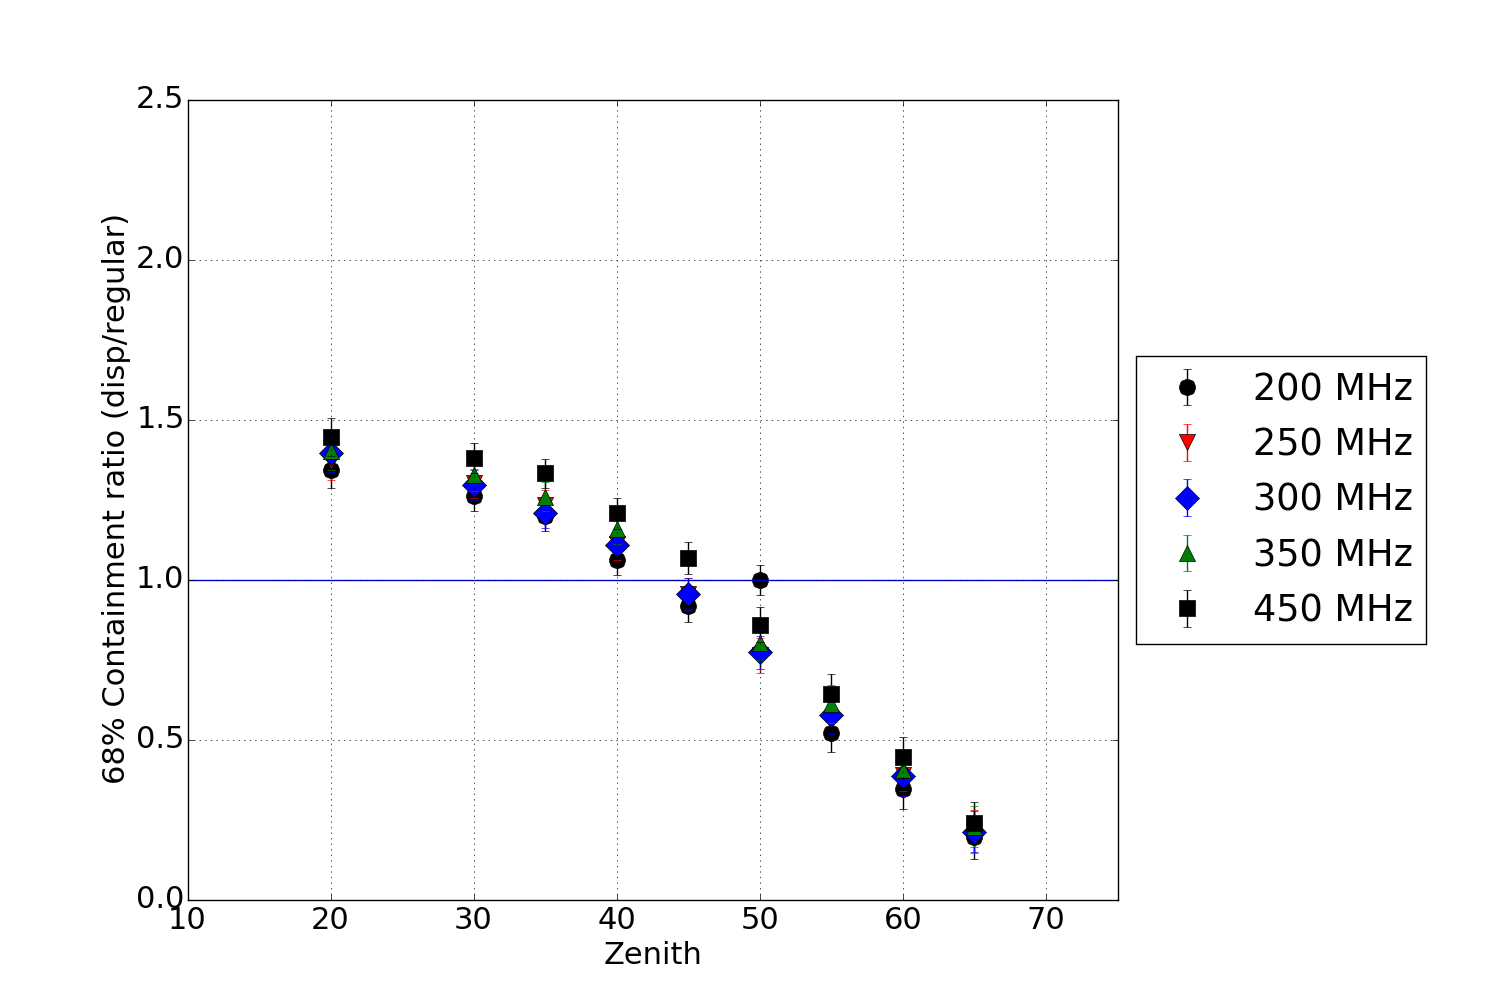
\includegraphics[width=0.8\linewidth]{images/disp_standard_ratio_xzen}
      \caption[``standard'' \disp table reconstruction]{Ratio of 68\% containment of the ``standard'' \disp table to that from Method0}  
      \label{fig:olddisp_ratio}
  \end{center}
\end{figure}

\begin{figure}[htbp]
  \centering
  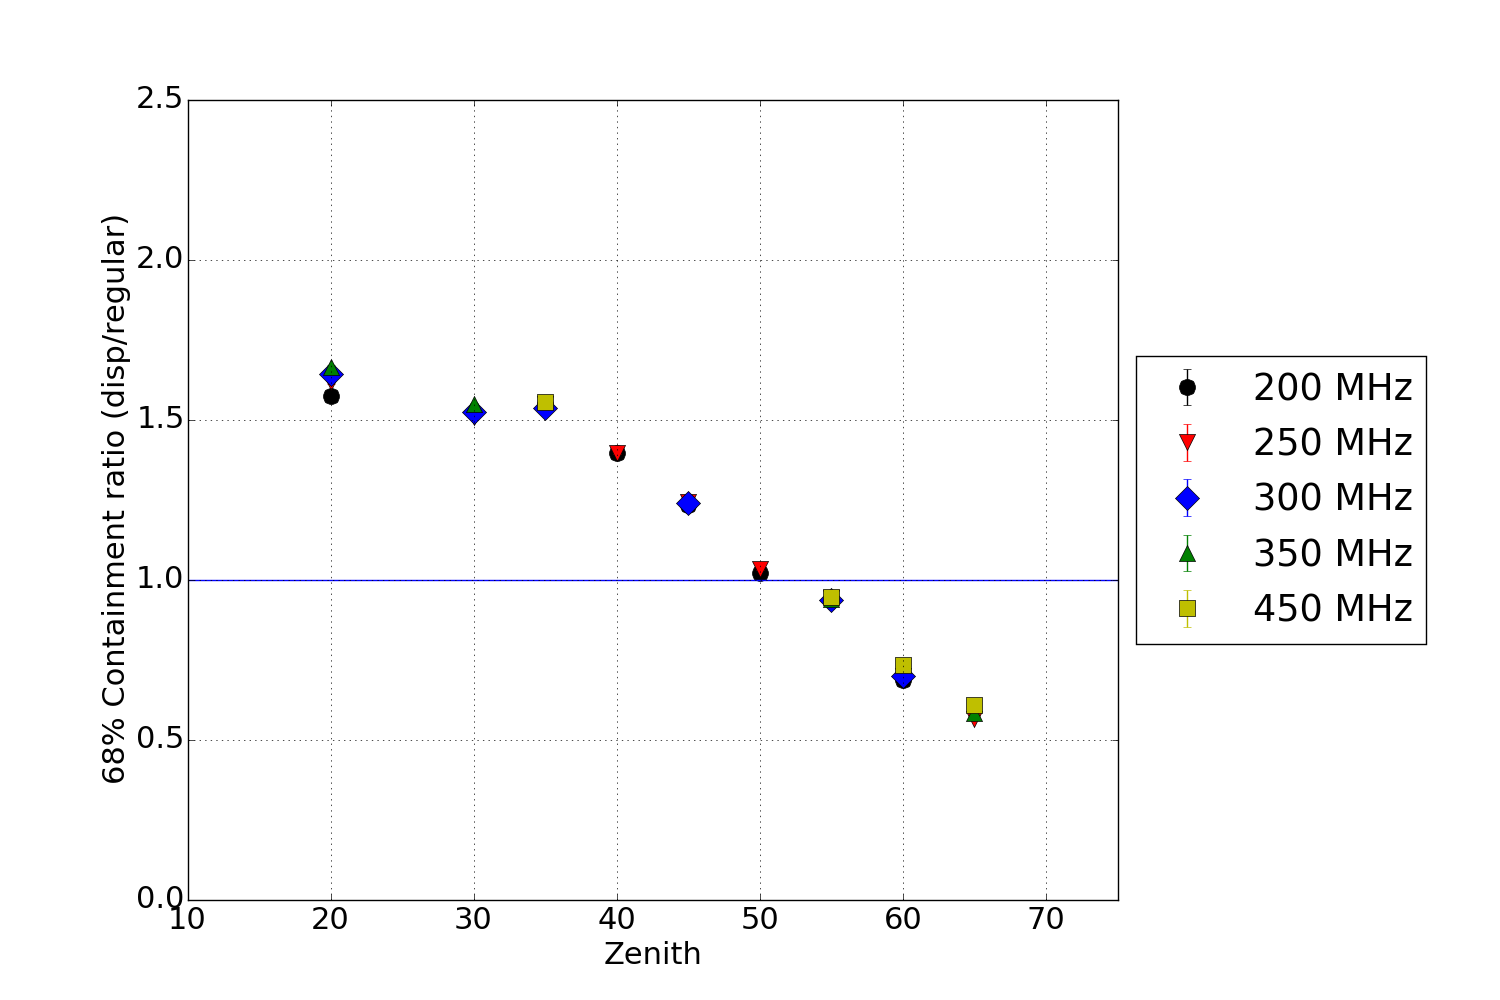
\includegraphics[width=0.8\linewidth]{images/disp_250_ratio_xzen}
  \caption[Test \disp table reconstruction (noise = $250$ MHz)]{Ratio of the 68\% containment from reconstruction using test \disp table ($\sim 1.9\e6$ events all at noise $= 250$ MHz) and that from Method0}
  \label{fig:disp_ratio_250}
\end{figure}

\subsection{Over-training}
BDT based regression is quite robust under non-linear correlations between discriminating parameters, however the primary vulnerability of this method, is that  to over-training - where the decision tree starts to be informed by noise and nuisance parameters in the training sample rather than relevant effects. This results in substantially different reconstruction efficiencies between training and testing samples. The ROOT TMVA package has a built-in test for over-training where it randomly selects a given fraction of the supplied events (for the purposes of this work, this fraction was taken to be 50\%) to use for testing. These events are then not used to train the regression trees and are instead used only to generate a measure of the over-training.
This check of the over-training for one of the test tables (noise $= 450$ MHz), shown in Fig. \ref{fig:overtraining}, demonstrates that there was no meaningful over-training of the table at least based on effects in the training sample.

There remains however, the possibility of effects related to noise level that might appear in the training \textit{and} testing samples (which are generated separately at each noise level), but not in observational data sets, which would be overlooked by this measure of over-training.

\begin{figure}[H]
  \centering
  \subfigure[Deviation of reconstructed \disp parameter from Monte-Carlo \disp parameter in training sample]{
    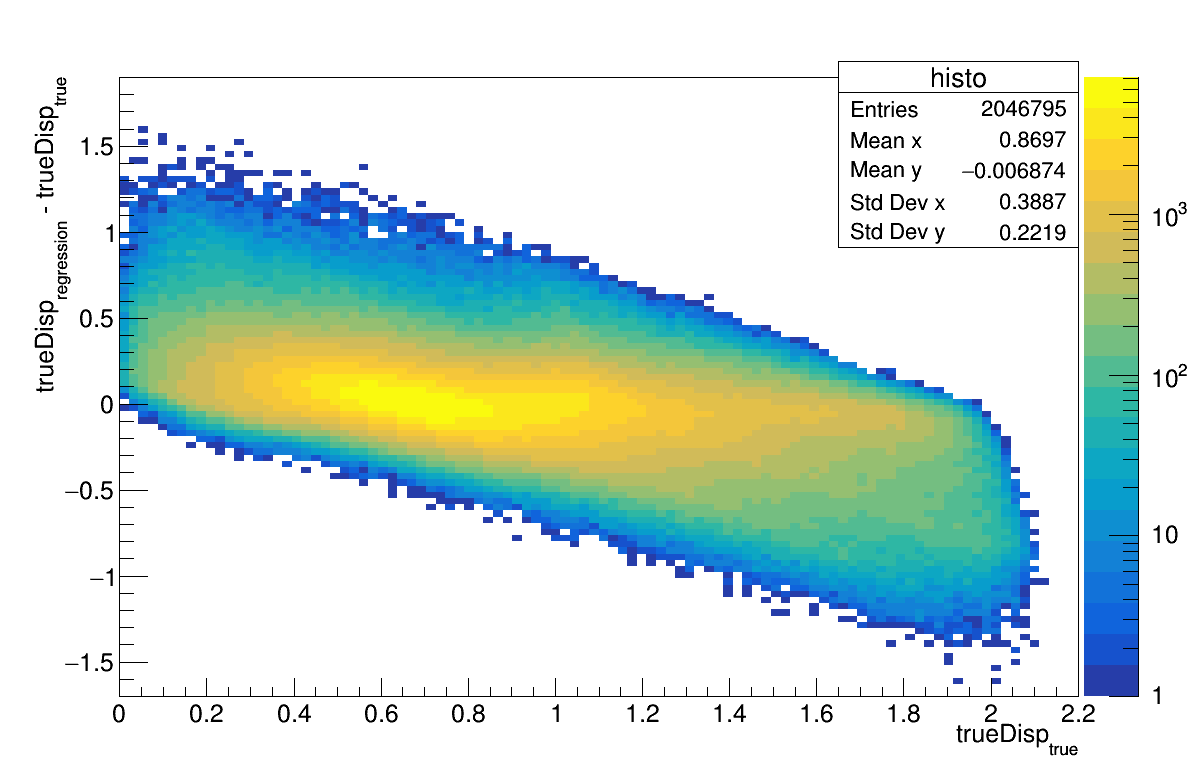
\includegraphics[width=.47\linewidth]{images/trueDisp_Train}
    \label{fig:disp_train_overtraining}
  }
  \subfigure[Deviation of reconstructed \disp parameter from Monte-Carlo \disp parameter in testing sample]{
    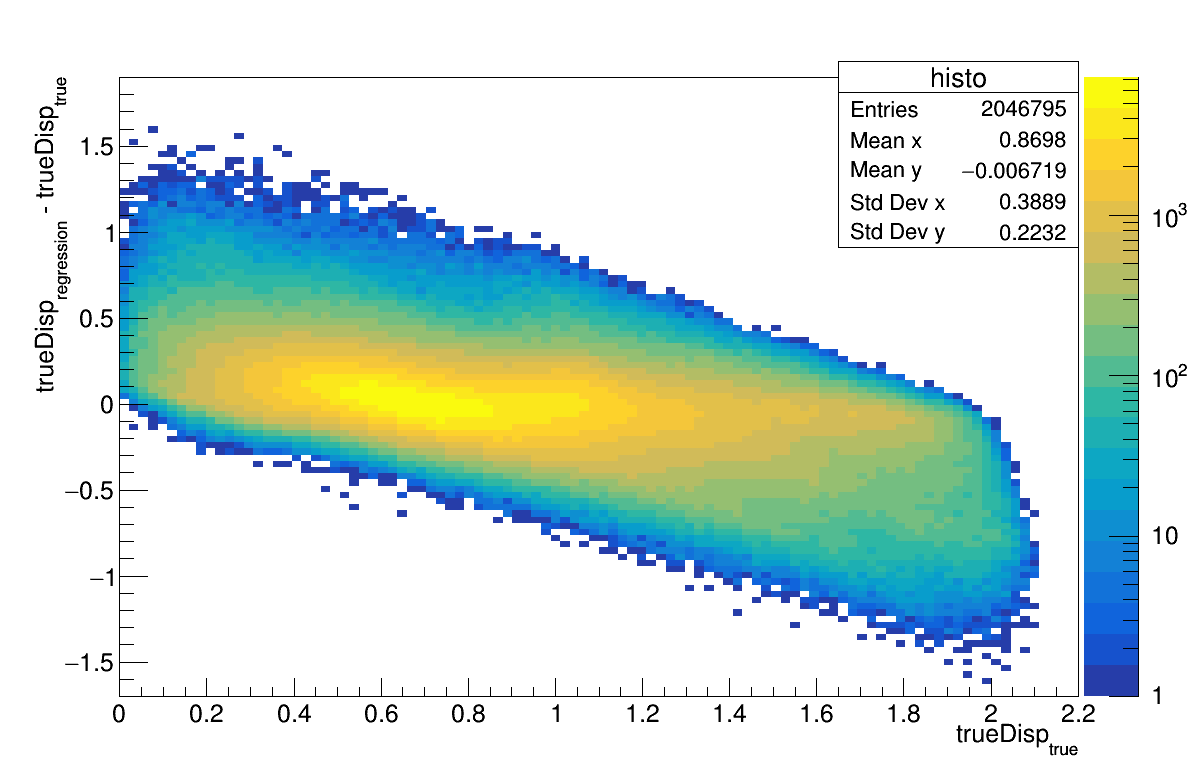
\includegraphics[width=.47\linewidth]{images/trueDisp_Test}
    \label{fig:disp_test_overtraining}
  }
  \subfigure[Deviation of reconstructed \disp Error parameter from Monte-Carlo \disp Error parameter in training sample]{
    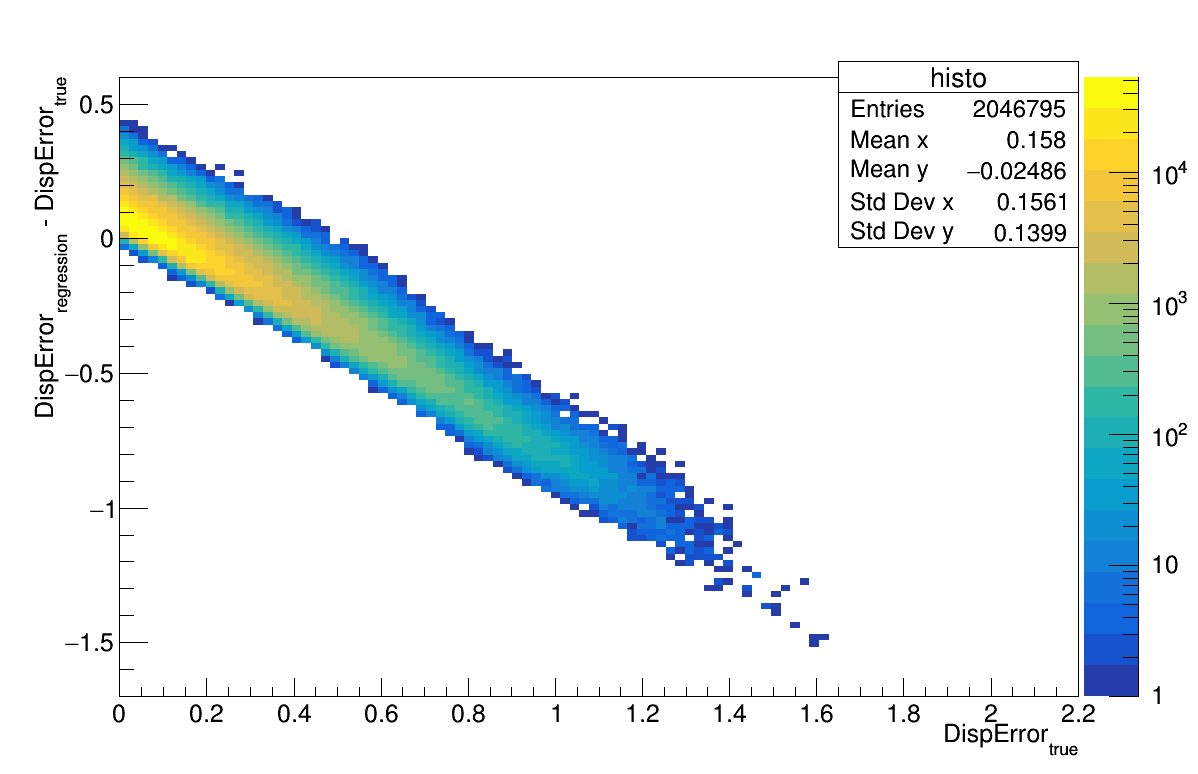
\includegraphics[width=.47\linewidth]{images/DispError_Train}
    \label{fig:dispErr_train_overtraining}
  }
  \subfigure[Deviation of reconstructed \disp Error parameter from Monte-Carlo \disp Error parameter in testing sample]{
    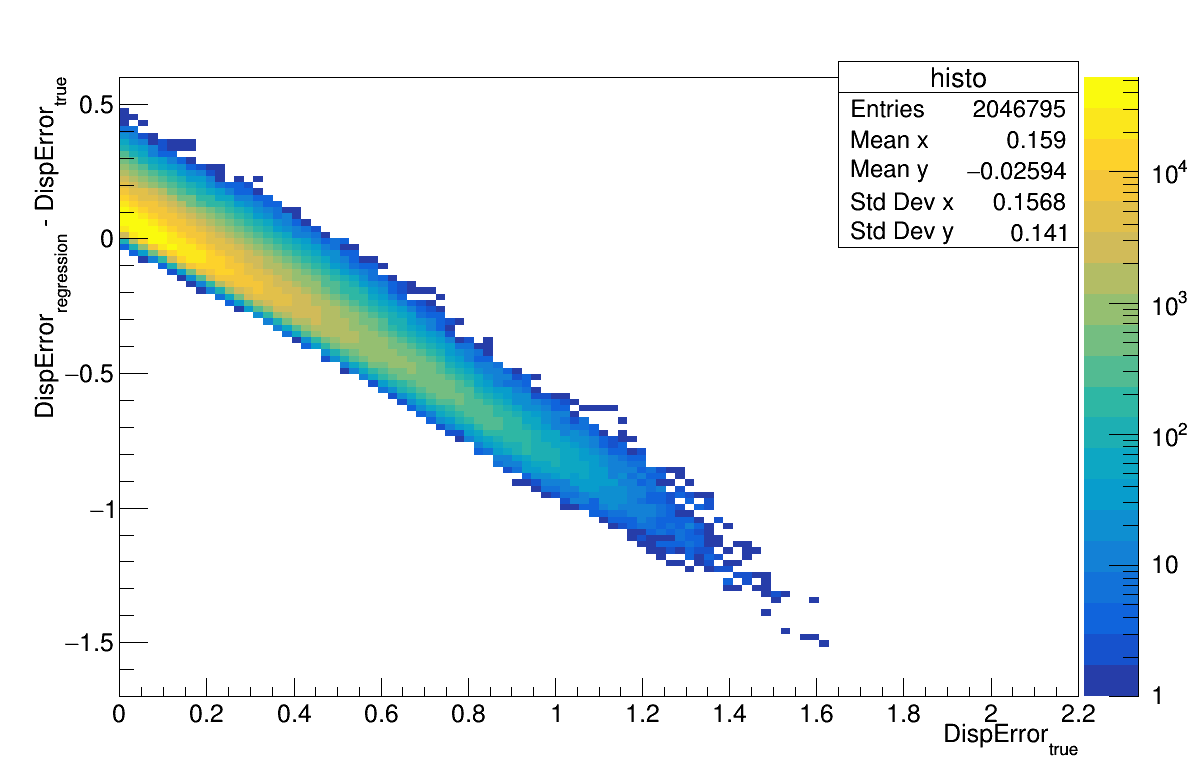
\includegraphics[width=.47\linewidth]{images/DispError_Test}
    \label{fig:dispErr_test_overtraining}
  }
  \subfigure[Deviation of reconstructed MAError parameter from Monte-Carlo MAError parameter in training sample]{
    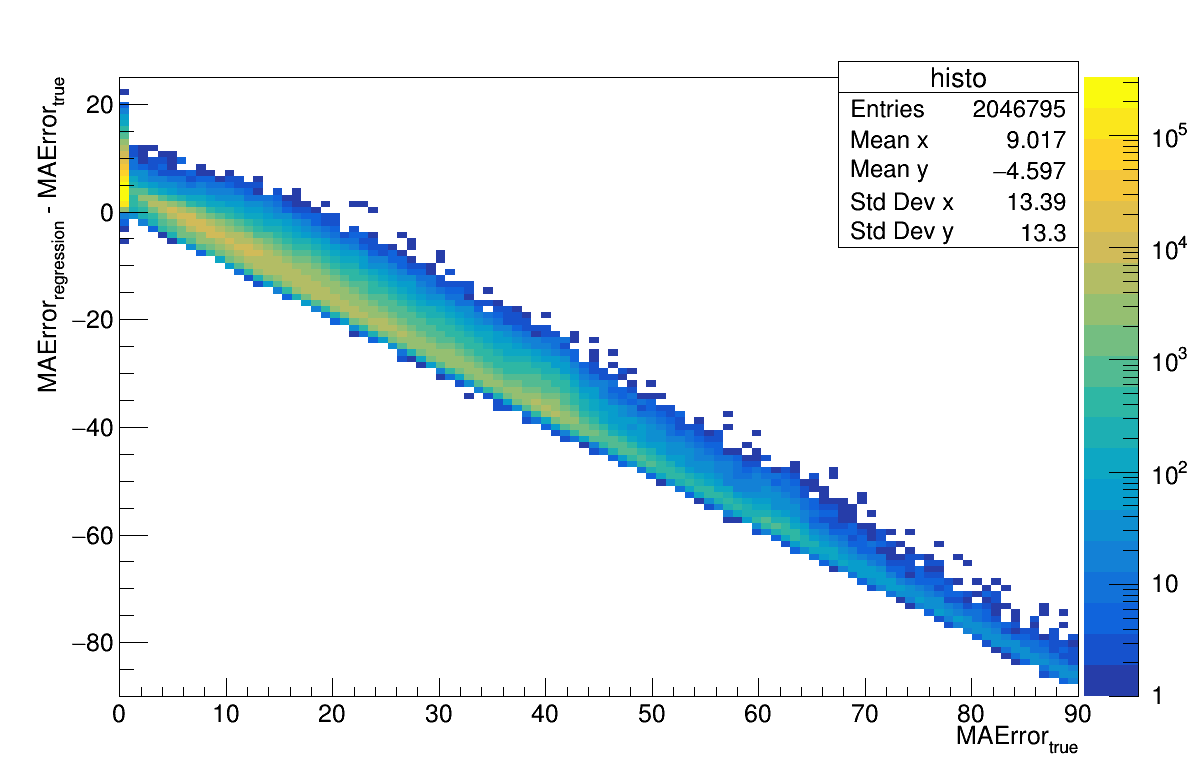
\includegraphics[width=.47\linewidth]{images/MAError_Train}
    \label{fig:MAErr_train_overtraining}
  }
  \subfigure[Deviation of reconstructed MAError parameter from Monte-Carlo MAError parameter in testing sample]{
    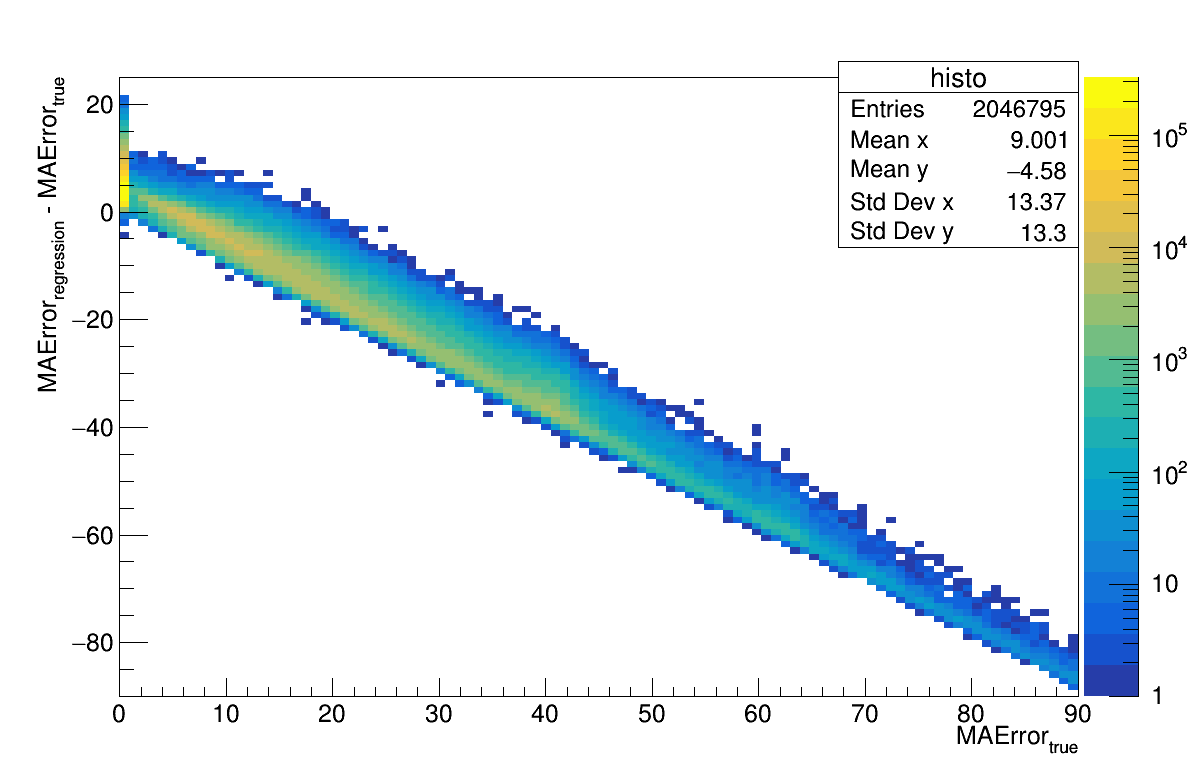
\includegraphics[width=.47\linewidth]{images/MAError_Test}
    \label{fig:MAErr_test_overtraining}
  }
  \caption[Over-training test]{Over-training check on reconstruction using a \disp table generated at a single noise level.}
  \label{fig:overtraining}
\end{figure}

\subsection{Noise Related Effects}
The first set of \disp tables was also generated at a single noise level ($250$ MHz), allowing us to test the dependence of the resolution of this method (as measured by 68\% containment) on noise level -- some kind of noise-dependent effect would suggest over-training that would not be evident from the testing sample in the ROOT TMVA method since all the data provided to the package would have been at the same noise level. A comparison of angular resolution across noise levels revealed no significant dependence of the 68\% containment on noise (see Fig. \ref{fig:olddisp_ratio}, \ref{fig:disp_ratio_250} and \ref{fig:disp_ratio_450}).

\begin{figure}[htbp]
  \centering
  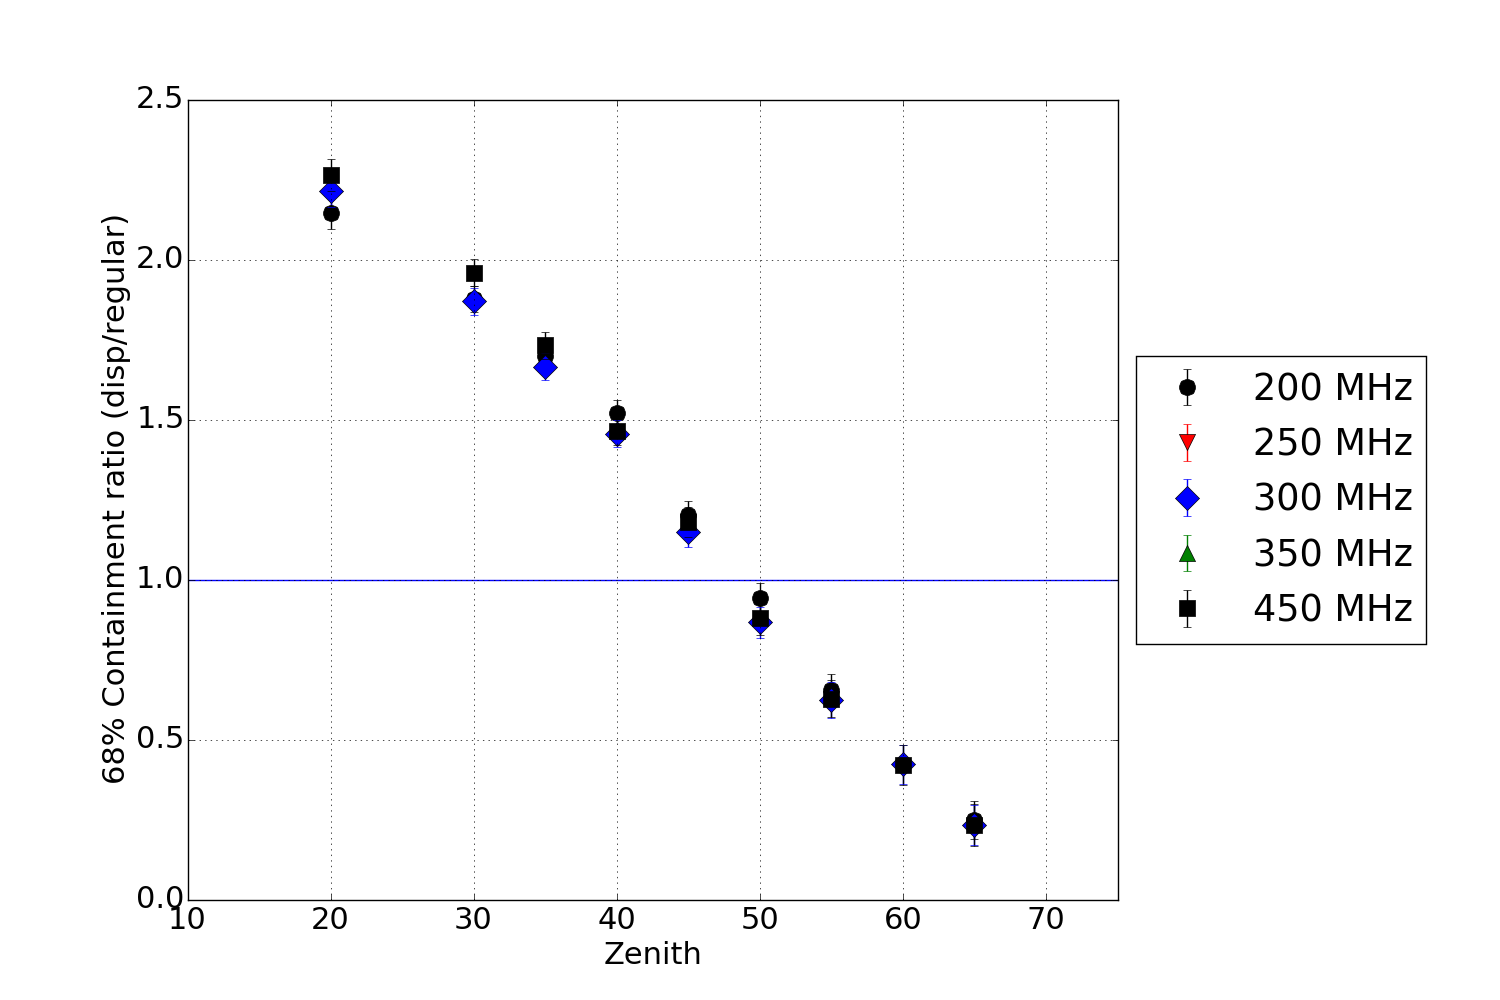
\includegraphics[width=0.8\linewidth]{images/disp_450_ratio_xzen}
  \caption[\disp table reconstruction vs noise]{Ratio of 68\% containment of the noise=450MHz \disp table ($\sim 2.1\e6$ events) to that from Method0}
  \label{fig:disp_ratio_450}
\end{figure}

A second set of test \disp tables was generated using a single noise level (noise $= 450$ MHz) to test for noise-related over-training (see Fig. \ref{fig:disp_ratio_450}). These tables performed slightly better than the first test tables and comparably to the standard \disp tables. Since the noise-related effects did not seem to play a significant role in reconstruction, noise was dropped as a discriminating parameter for further analysis.

To generate a set of \disp tables with better angular resolution (as measured by 68\% containment), another set of \disp tables was trained on a larger number of simulations across zenith angles (as before) as well as across the noise spectrum.

\subsection{Higher Statistics Tables}
Once it was determined that there was no significant over-training in the small sample \disp tables, and the noise level had little bearing on the 68\% containment measure of the reconstruction, it was determined that different noise level simulation events could be used as independent training events to have a higher statistics \disp table, and make small improvements on the statistical uncertainty on the reconstruction. The simulation data from across the noise spectrum and zenith range was used to generate a \disp table that sampled the entire parameter space more exhaustively.

A new set of \disp tables was generated with a training sample four times that of the initial test tables. The improvements in resolution due to change in sample size were modest, and confined to the range of zenith angles where the standard method outperforms the \disp method quite considerably.

\begin{figure}[htbp]
  \centering
  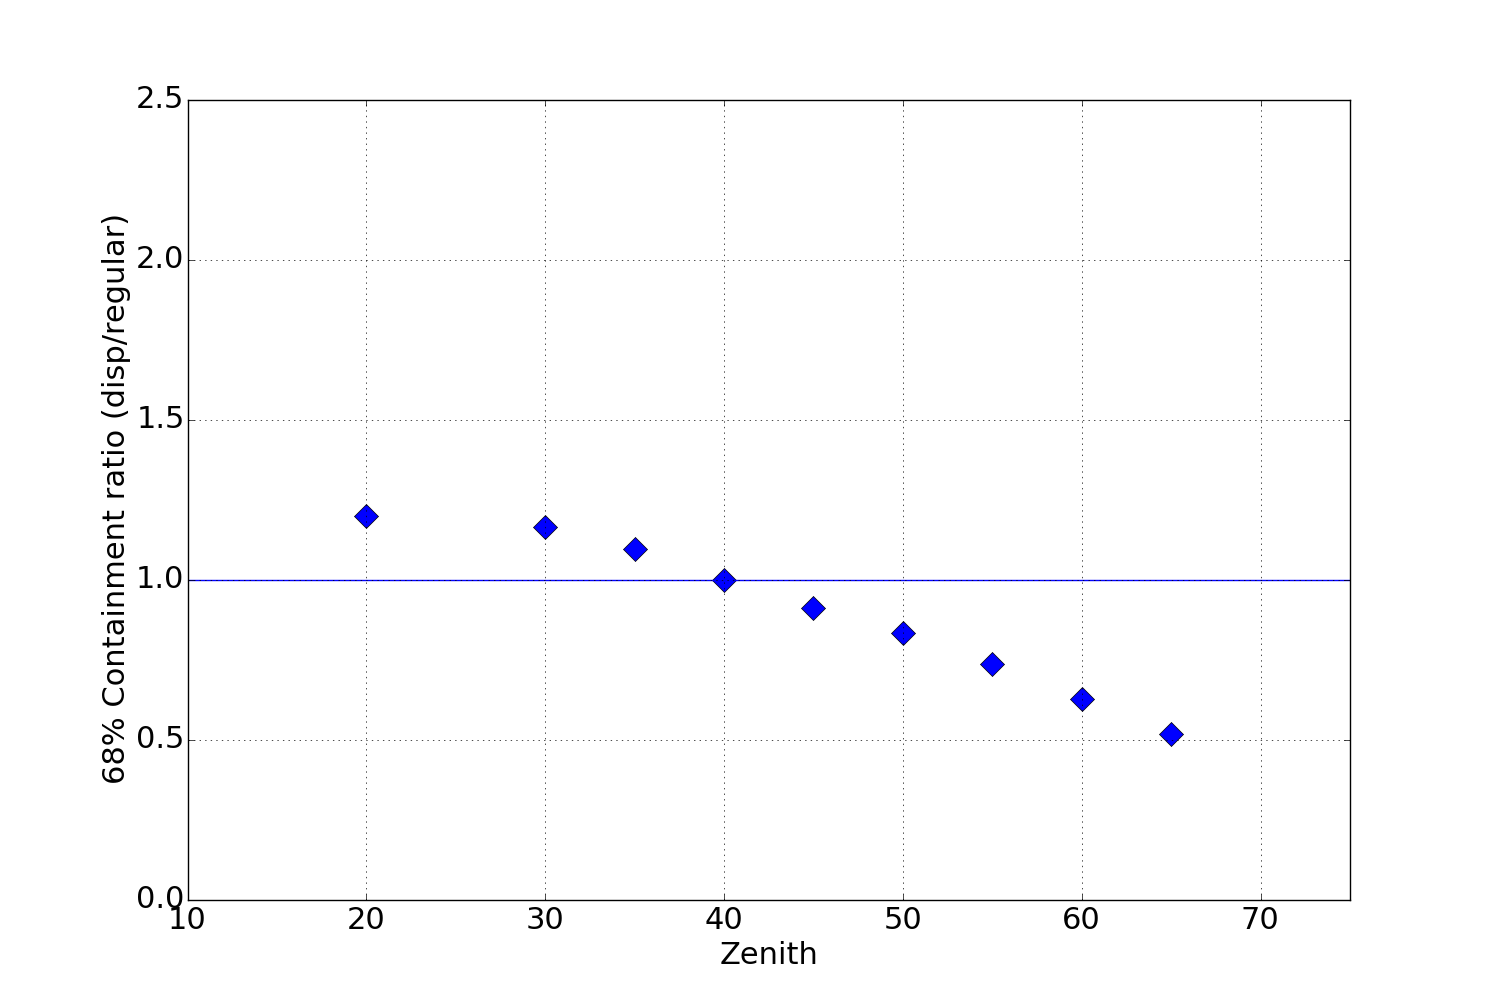
\includegraphics[width=0.8\linewidth]{images/disp_450x4size_ratio_xzen}
  \caption[\disp table reconstruction vs noise]{Ratio of 68\% containment of the noise=450MHz \disp table ($\sim 8.4\e6$ events) to that from Method0}
  \label{fig:disp_ratio_450x4}
\end{figure}


\end{document}

